\documentclass{article}
\usepackage[utf8]{inputenc}
\usepackage[italian]{babel}
\usepackage{amsmath}
\usepackage{amssymb}
\usepackage{siunitx}
\usepackage{tabularray}
\usepackage{graphicx}
\usepackage{float}
\usepackage{minted}
\usepackage[page]{appendix}
\newcommand*{\diam}{\varnothing}
\newcommand*{\best}[1]{{#1}_\text{best}}
\newcommand*{\bestp}[1]{{\left(#1\right)}_\text{best}}
\newcommand*{\pbest}[1]{\left({#1}_\text{best}\right)}
\newcommand*{\pbestp}[1]{\left({\left(#1\right)}_\text{best}\right)}
\newcommand*{\errrel}[1]{\frac{\delta #1}{{#1}_\text{best}}}
\newcommand*{\Th}{^{232}_{\;\;90} \text{Th}}
\title{
    Laboratorio di Fisica 1\\
    R4: Misura di variabili aleatorie
}
\author{Gruppo 17: Bergamaschi Riccardo, Graiani Elia, Moglia Simone}
\date{8/11/2023 – 15/11/2023}
\makeindex
\begin{document}

\maketitle

\begin{abstract}
    Il gruppo di lavoro ha misurato due variabili aleatorie, osservando come queste
    rispecchino le rispettive distribuzioni teoriche (di Bernoulli e di Poisson).
\end{abstract}

\section{Processo di Bernoulli}

\subsection{Dati sperimentali}
Eseguiamo 400 lanci di sei dadi distinti\footnote{Li distinguiamo in base al colore},
registrandone tutti i risultati.
Per ogni possibile risultato, possiamo così
definire una variabile aleatoria\footnote{
    \emph{Notazione.} Per noi $0\in\mathbb{N}$.
} $s\in\left[1;6\right]\cap\mathbb{N}$
$x_s\in\left[0;6\right]\cap\mathbb{N}$ come il
numero di dadi, fra i sei lanciati, con risultato pari ad $s$.
Possiamo considerare il lancio dei sei dadi come un processo di Bernoulli,
in quanto i risultati dei dadi sono indipendenti fra loro. Di conseguenza,
la distribuzione di probabilità di $x_s$ è data da:
\[
    p \left(x_s=k\right) =
        \binom{6}{k}
        \left(\frac{1}{6}\right)^k
        \left(\frac{5}{6}\right)^{6-k}
        \qquad\forall k\in\left[0;6\right]\cap\mathbb{N}
\]
Di seguito riportiamo gli istogrammi dei dati così raccolti, assieme ai valori attesi,
calcolati mediante la distribuzione teorica.

% \subsubsection*{Onestà dei dadi}
% Avendo segnato tutti i risultati di ogni dado, possiamo inoltre stimare se i dadi che
% abbiamo utilizzato sono truccati o meno. Infatti, su un dado onesto ci aspettiamo
% che escano tutti i risultati possibili con equa probabilità. Di seguito riportiamo
% gli istogrammi dei valori usciti su ogni dado.

% \begin{figure*}
%     \caption{...}
% \end{figure*}

\subsection{Simulazione}
Tramite un programma da noi scritto e compilato\footnote{\emph{Vedi} Appendice 1},
simuliamo la stessa esperienza con $10^{12}$ lanci dei sei dadi, al fine di
verificare la legge dei grandi numeri. Quest'ultima consiste nella tesi che,
su un grande numero di prove, i risultati si avvicinino, in proporzione,
ai valori attesi.

Di seguito riportiamo, in un istogramma, i risultati della simulazione.

\pagebreak
\section{Processo di Poisson}
\subsection{Materiali e strumenti di misura utilizzati}
\begin{center}
    \begin{tblr}{ |Q[l,m]|Q[c,m]|Q[c,m]|Q[c,m]| }
        \hline
        \textbf{Strumento di misura} & \textbf{\:\:\:\:\:Soglia\:\:\:\:\:} & \textbf{Portata} & \textbf{Sensibilità} \\
        \hline
        {Contatore Geiger} & \qty{1}{conteggi \per s} & N./A. & \qty{1}{conteggi \per s} \\
        \hline[dashed]
        Metro a nastro & \qty{0.1}{cm} & \qty{300.0}{cm} & \qty{0.1}{cm} \\
        \hline
        \hline
        \textbf{Altro} & \SetCell[c=3]{l} \textbf{Descrizione/Note} \\
        \hline
        {Campione di $\Th$} & \SetCell[c=3]{l} {
            Componente di una lampada da campeggio
        } \\
        \hline
    \end{tblr}
\end{center}


\subsection{Esperienza e procedimento di misura}

Per ogni distanza $d_i$ tra il campione di $\Th$ e il contatore Geiger
(con $i\in\left[1;4\right]\cap\mathbb{N}$), il gruppo di lavoro ha acquisito
i conteggi di raggi $\gamma$ emessi nella direzione del contatore ogni secondo
per un tempo complessivo di circa un'ora ($\qty{3657}{s}$)\footnote{
    Abbiamo scelto di acquisire esattamente 3657 secondi in quanto
    $3657$ minimizza la funzione
    $f(x)=\left\{\frac{x}{\pi}\right\}=\frac{x}{\pi} - \left\lfloor\frac{x}{\pi}\right\rfloor$
    meglio di $3600$.
}.

Infine, il gruppo di lavoro ha acquisito, sempre per $\qty{3657}{s}$,
i conteggi al secondo di raggi $\gamma$ nella direzione opposta rispetto
al campione,
per avere una stima della radioattività ambientale.

\emph{
    \textbf{Notazione.} Indichiamo con $\gamma_i$ complessivamente i conteggi
    acquisiti a distanza $d_i$ dal campione (con $i\in\left[1;4\right]\cap\mathbb{N}$),
    mentre con $\gamma_{t,i}$ il numero di conteggi nell'intervallo temporale
    $\left[(t-1)\;\unit{s};t\;\unit{s}\right]$ dall'inizio dell'acquisizione (con
    $t\in\left[1;3657\right]\cap\mathbb{N}$).
    Allora $\overline{\gamma_i}$ sarà la media della distribuzione, dove
    $\bestp{\overline{\gamma_i}}$ sarà la media dei conteggi,
    mentre $\sigma_{\gamma_i}$ sarà la deviazione standard e
    $
        \delta\!\left(\overline{\gamma_i}\right) =
        \sigma_{\overline{\gamma_i}} =
        \frac{\sigma_{\gamma_i}}{\sqrt{3657}}
    $
    l'errore sulla media.
    Analogamente per \emph{
        $\gamma_\text{amb}$,
        $\gamma_\text{amb}$ e
        $\overline{\gamma_\text{amb}}$.
    }
}

Di seguito, riportiamo le distribuzioni di tutti i $\gamma_i$
e la regerssione lineare dei conteggi in funzione di $1/d_i^2$.

\begin{center}
    \begin{figure}[H]
        % trim={< v > ^}
        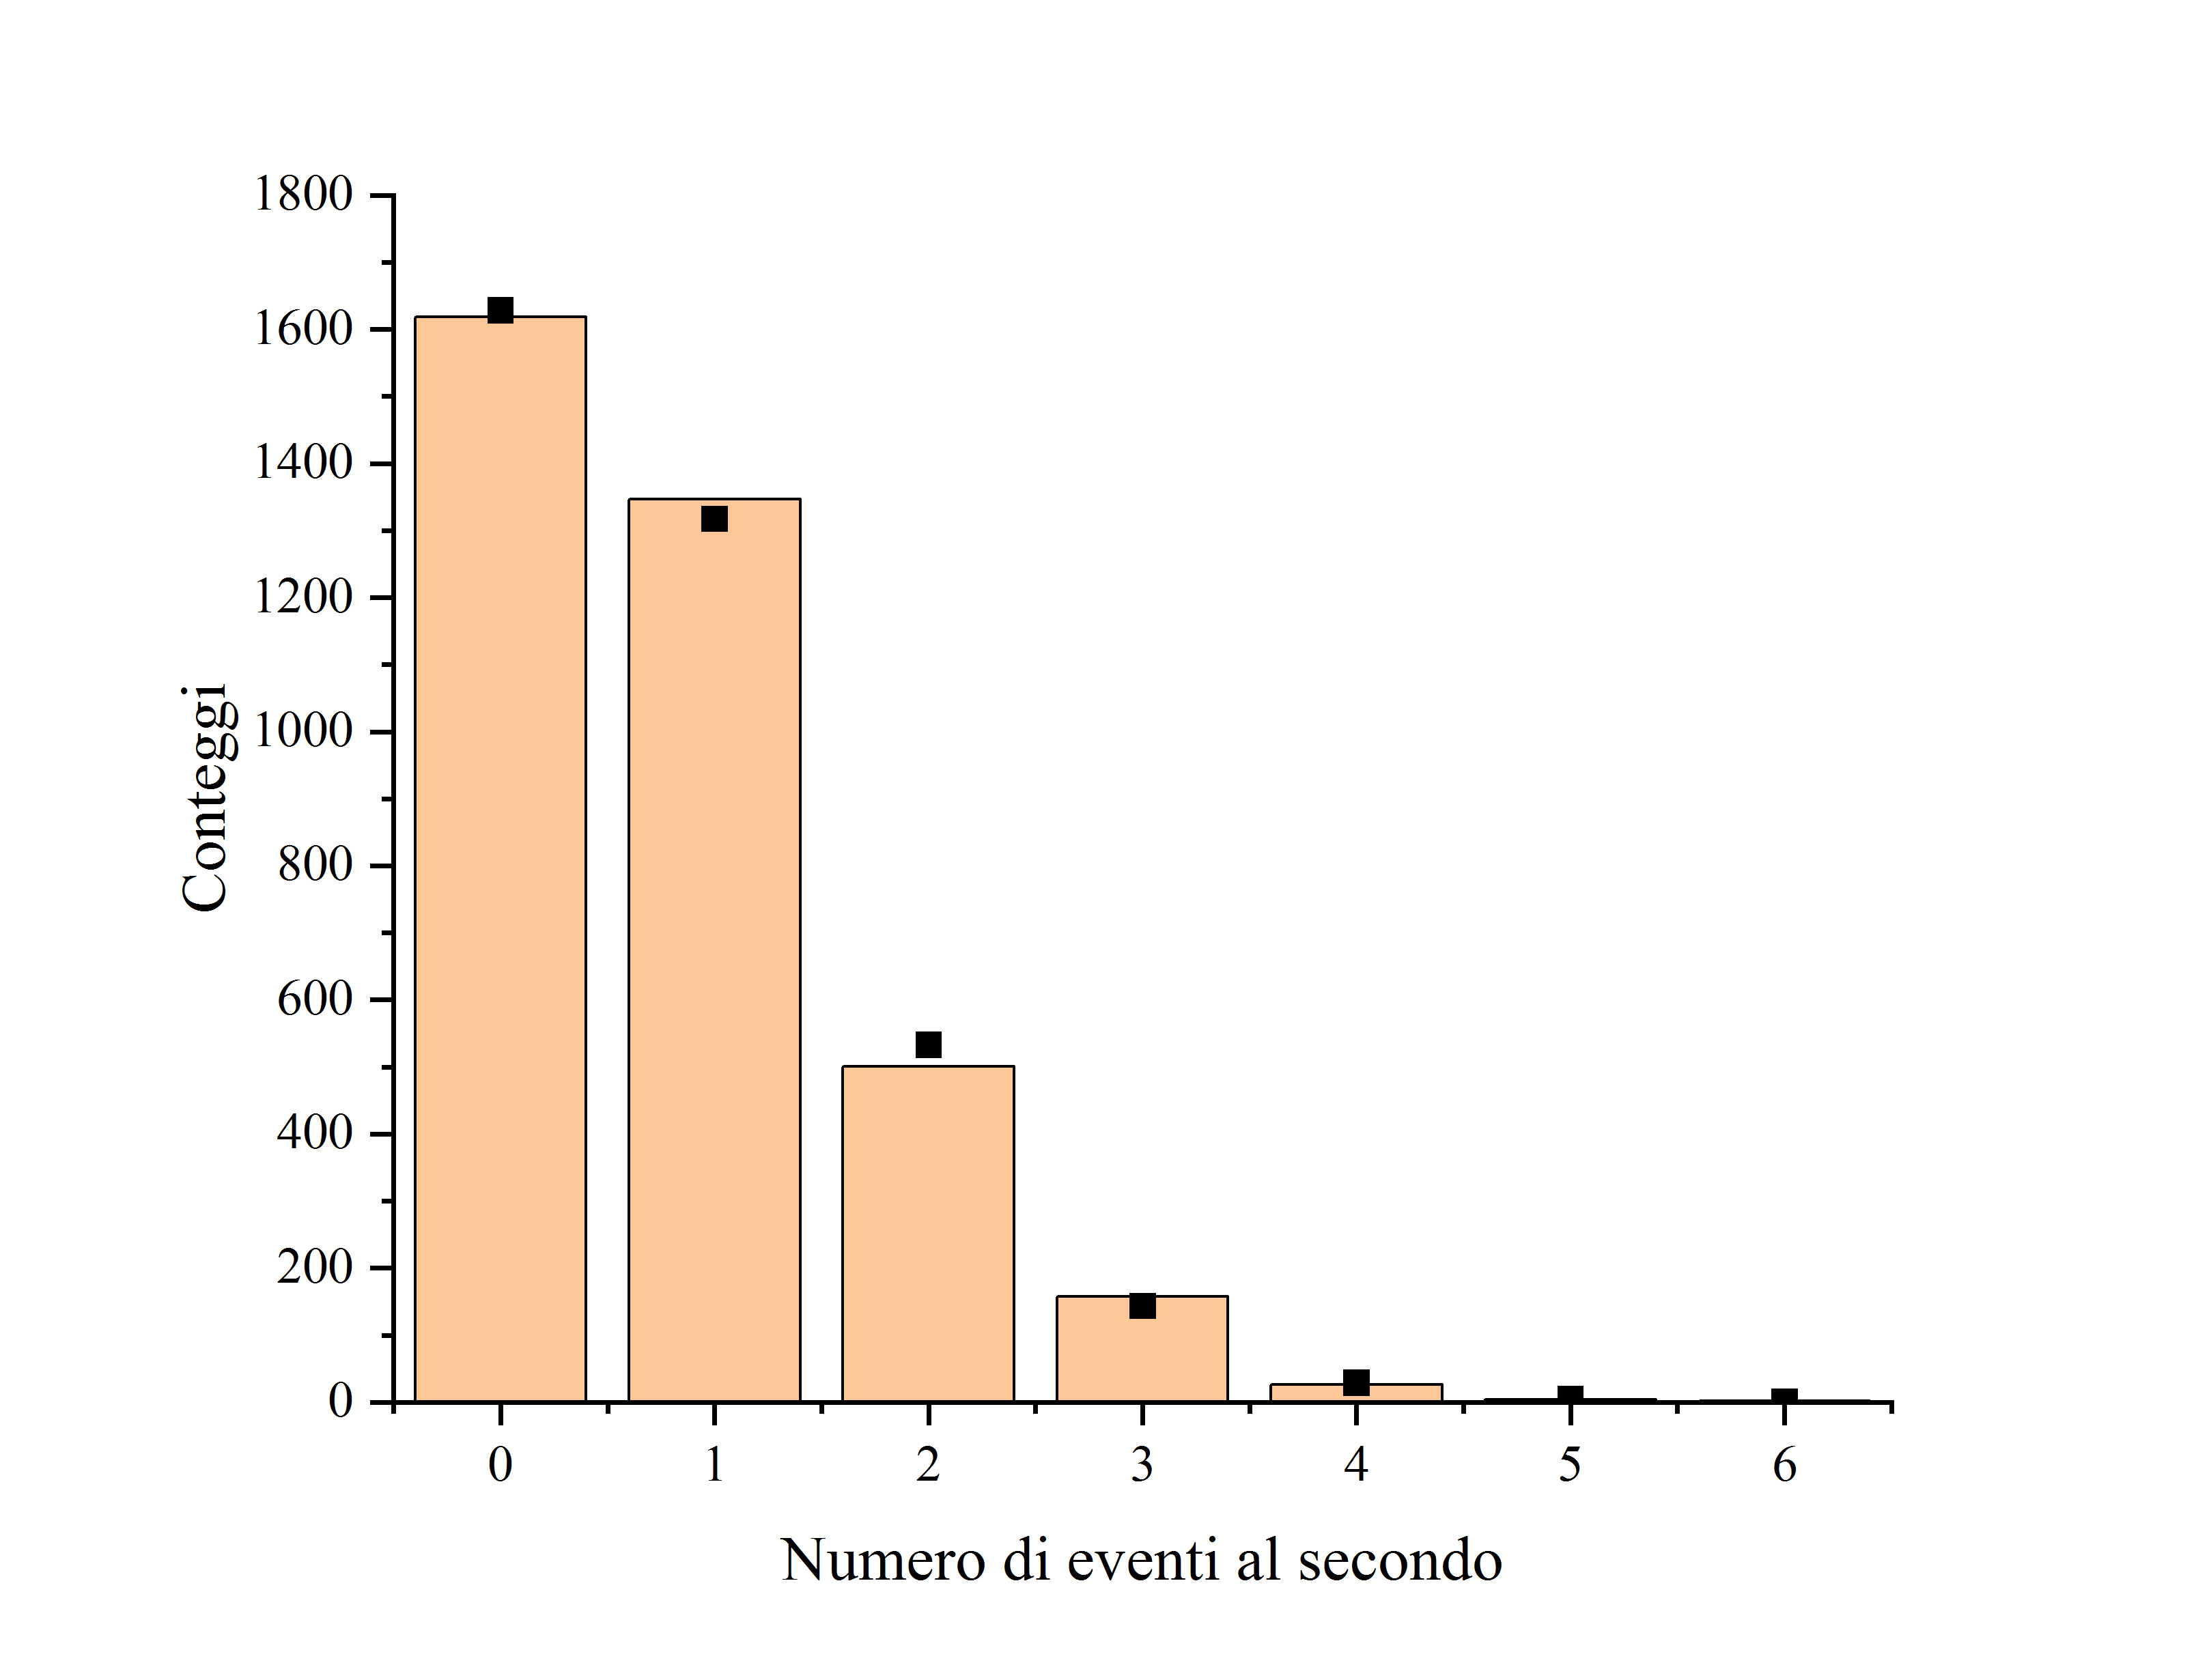
\includegraphics[trim={2cm .5cm 2.4cm 2.1cm},clip,width=.5\textwidth]{img/Geiger2.jpg}
        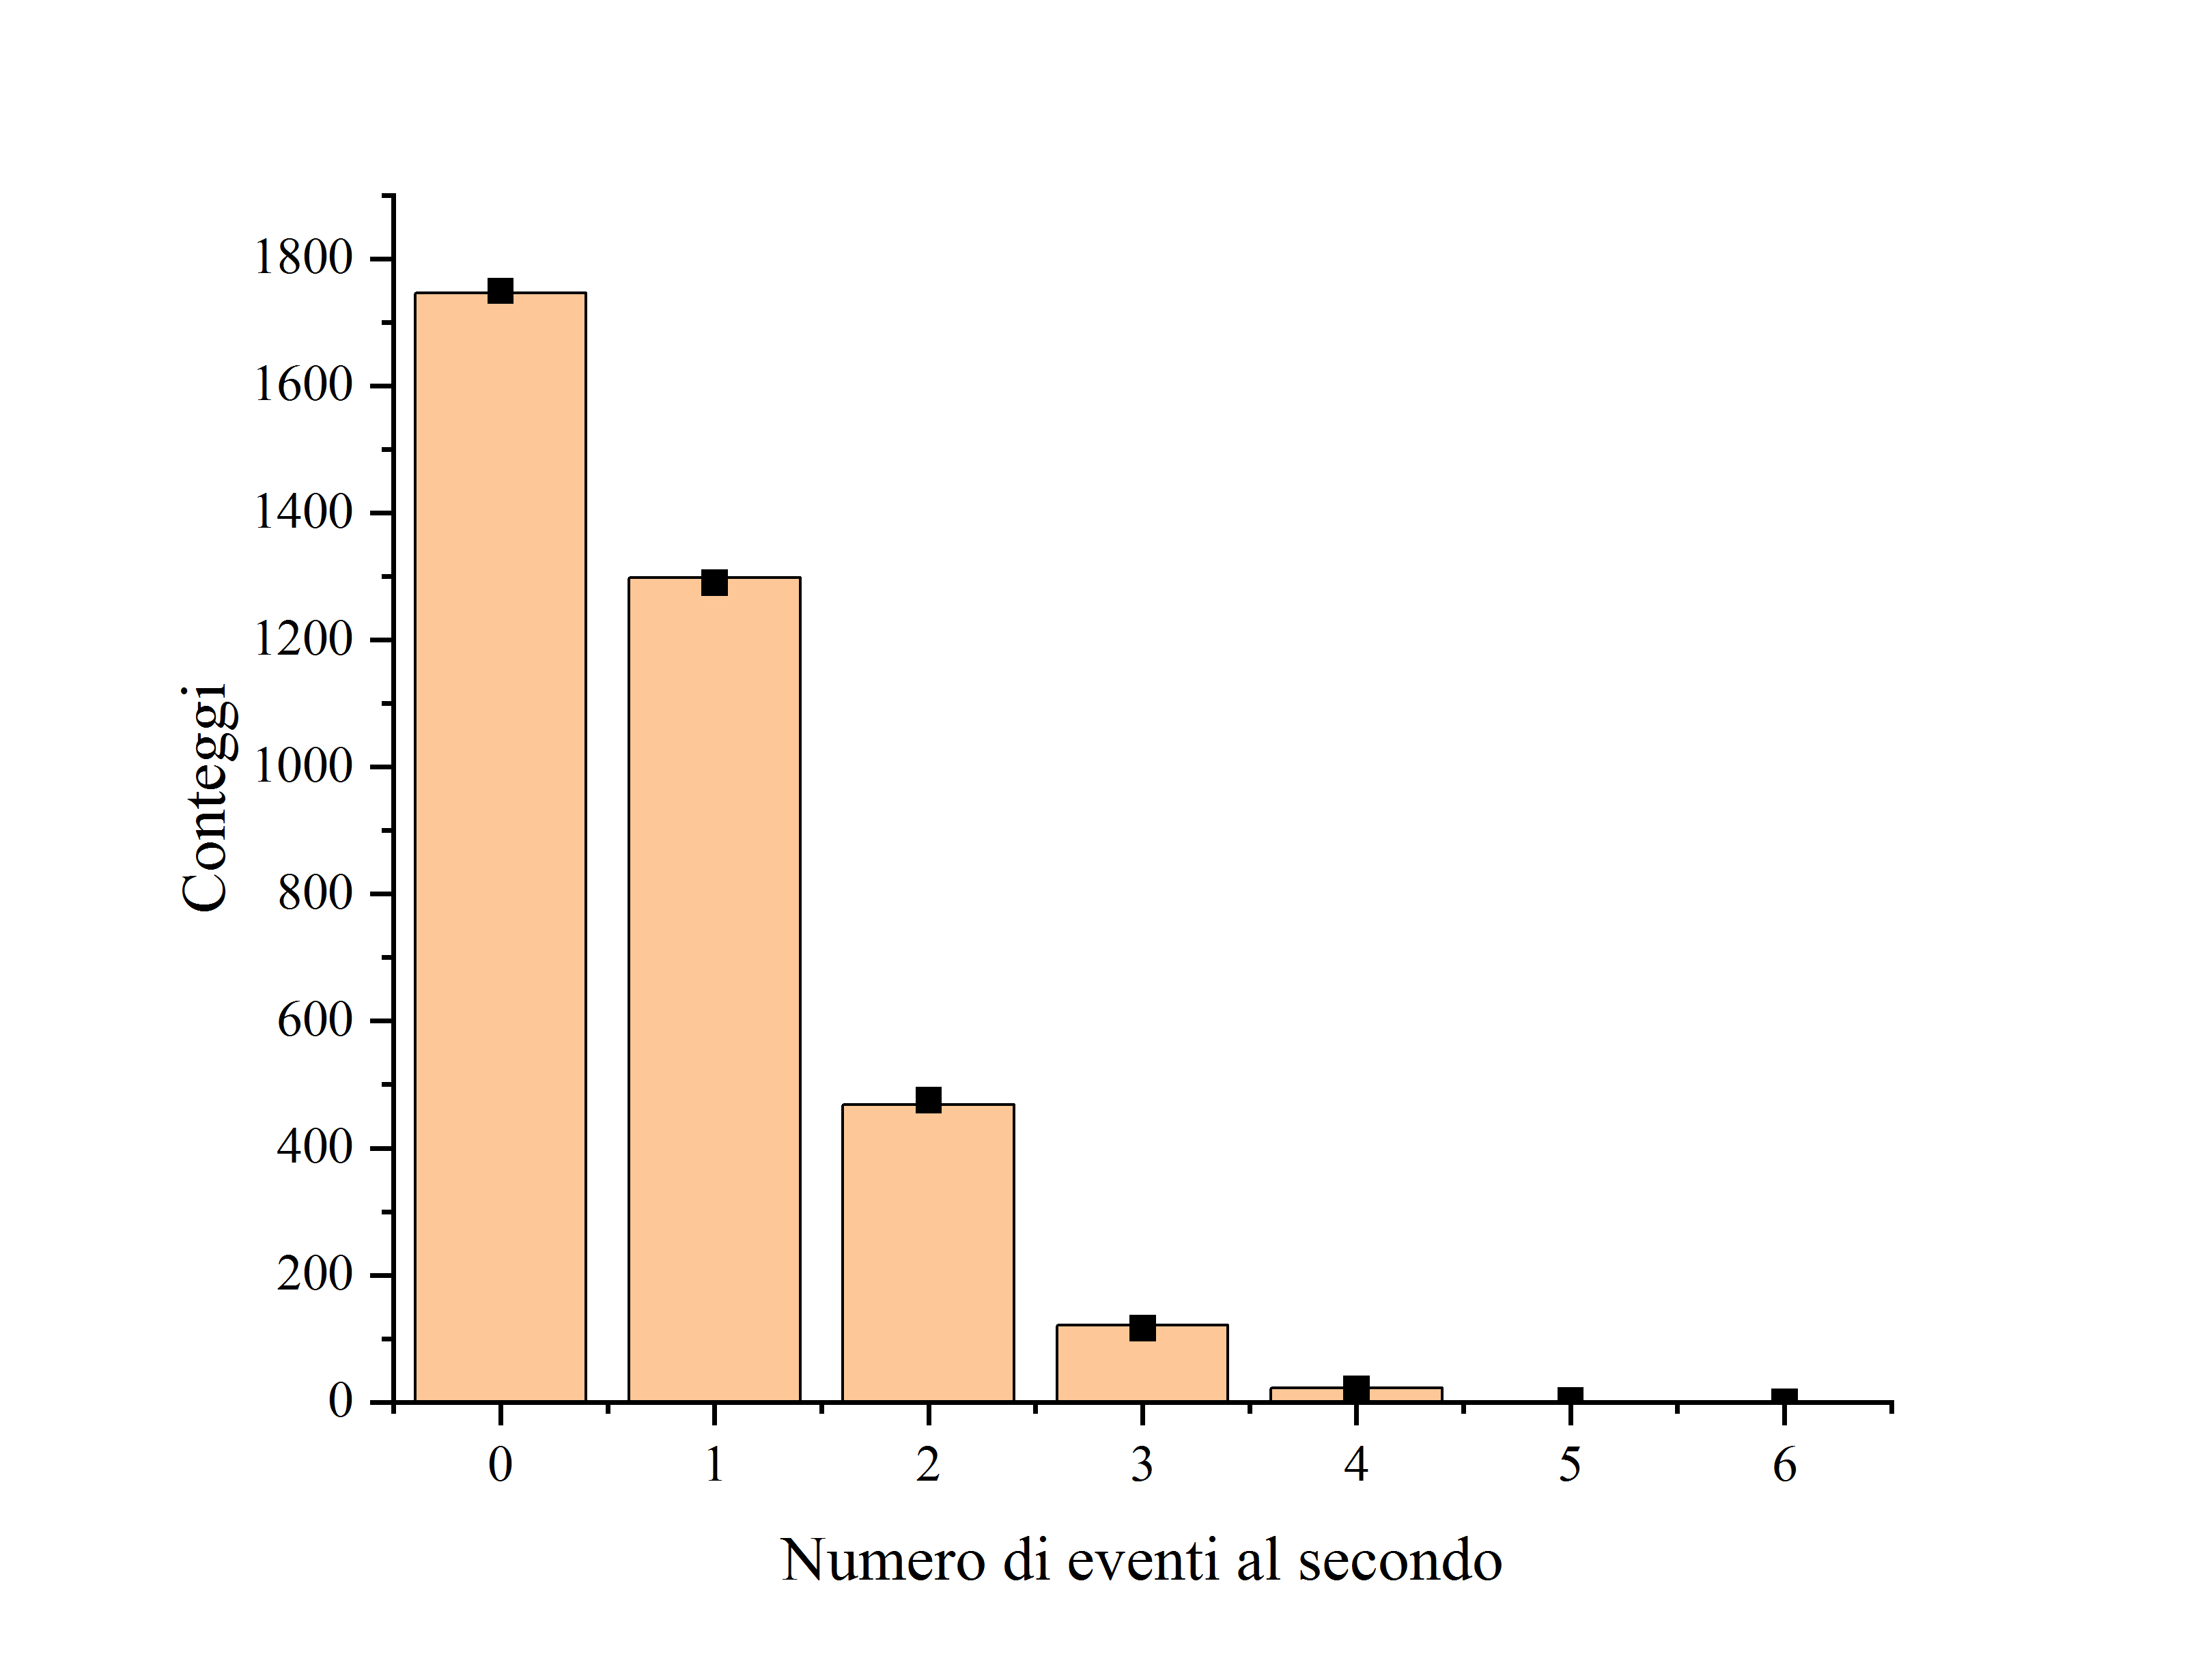
\includegraphics[trim={2cm .5cm 2.4cm 2.1cm},clip,width=.5\textwidth]{img/Geiger1.jpg}
        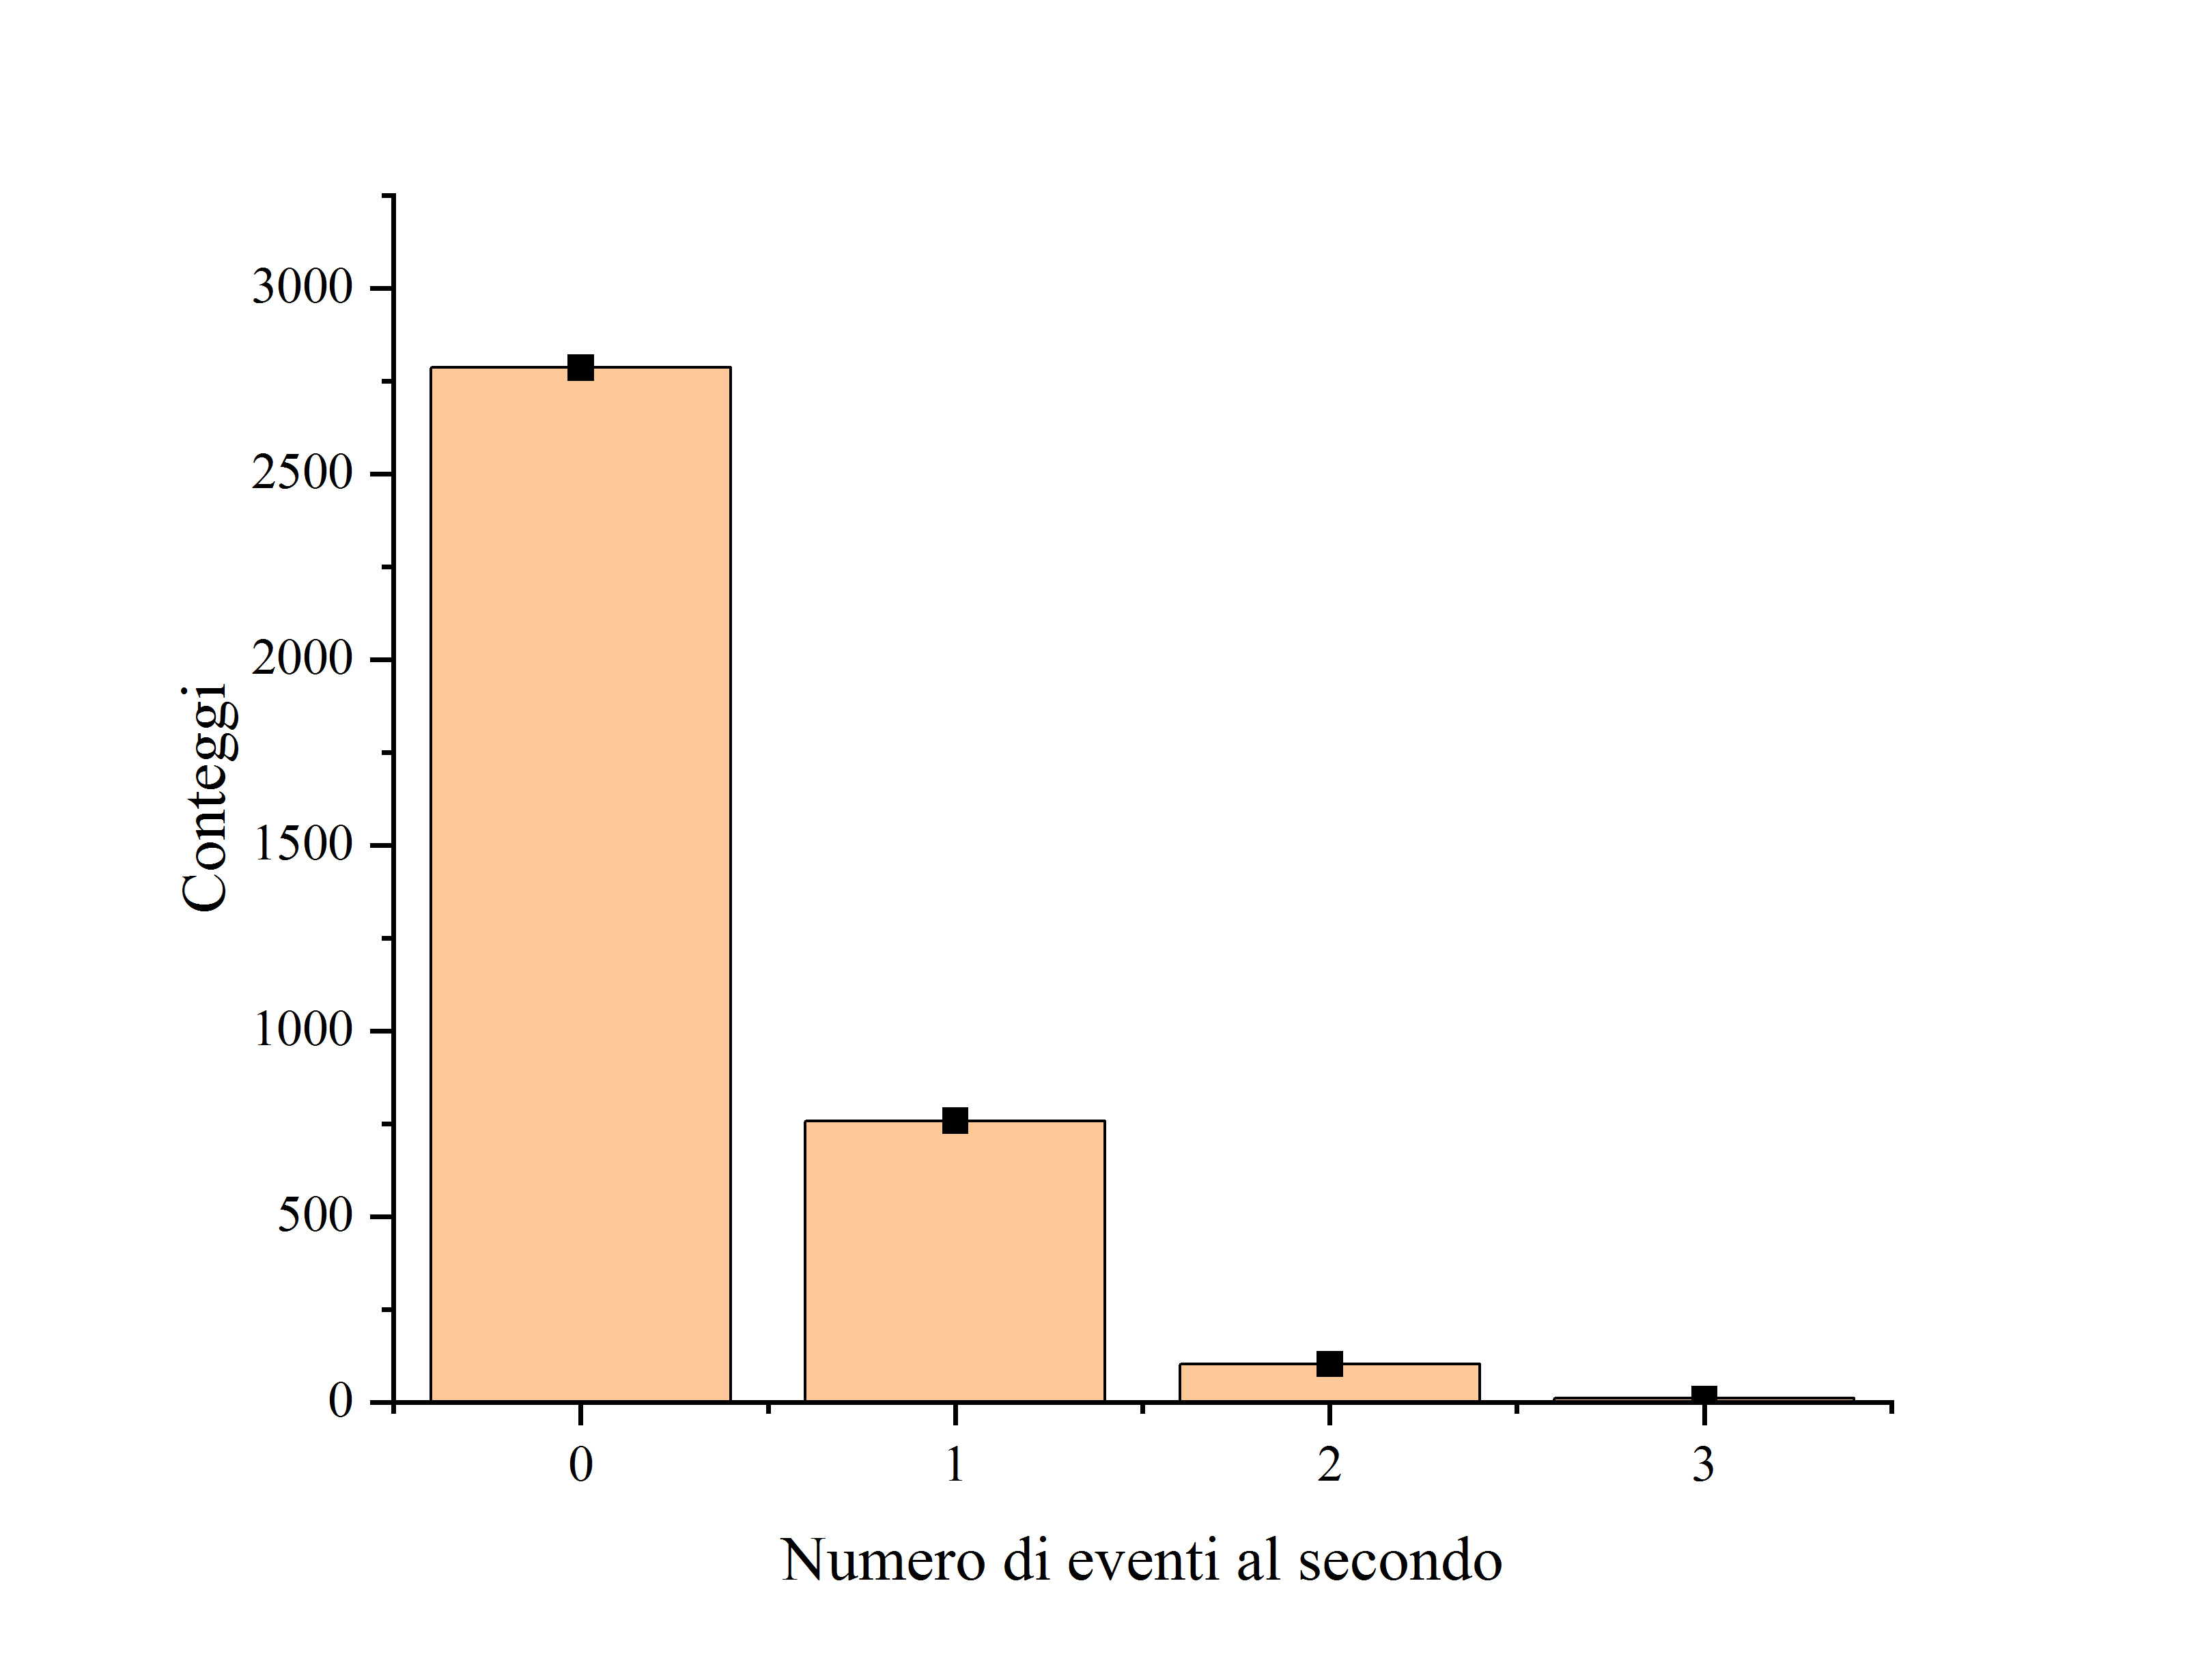
\includegraphics[trim={2cm .5cm 2.4cm 2.1cm},clip,width=.5\textwidth]{img/Geiger4.jpg}
        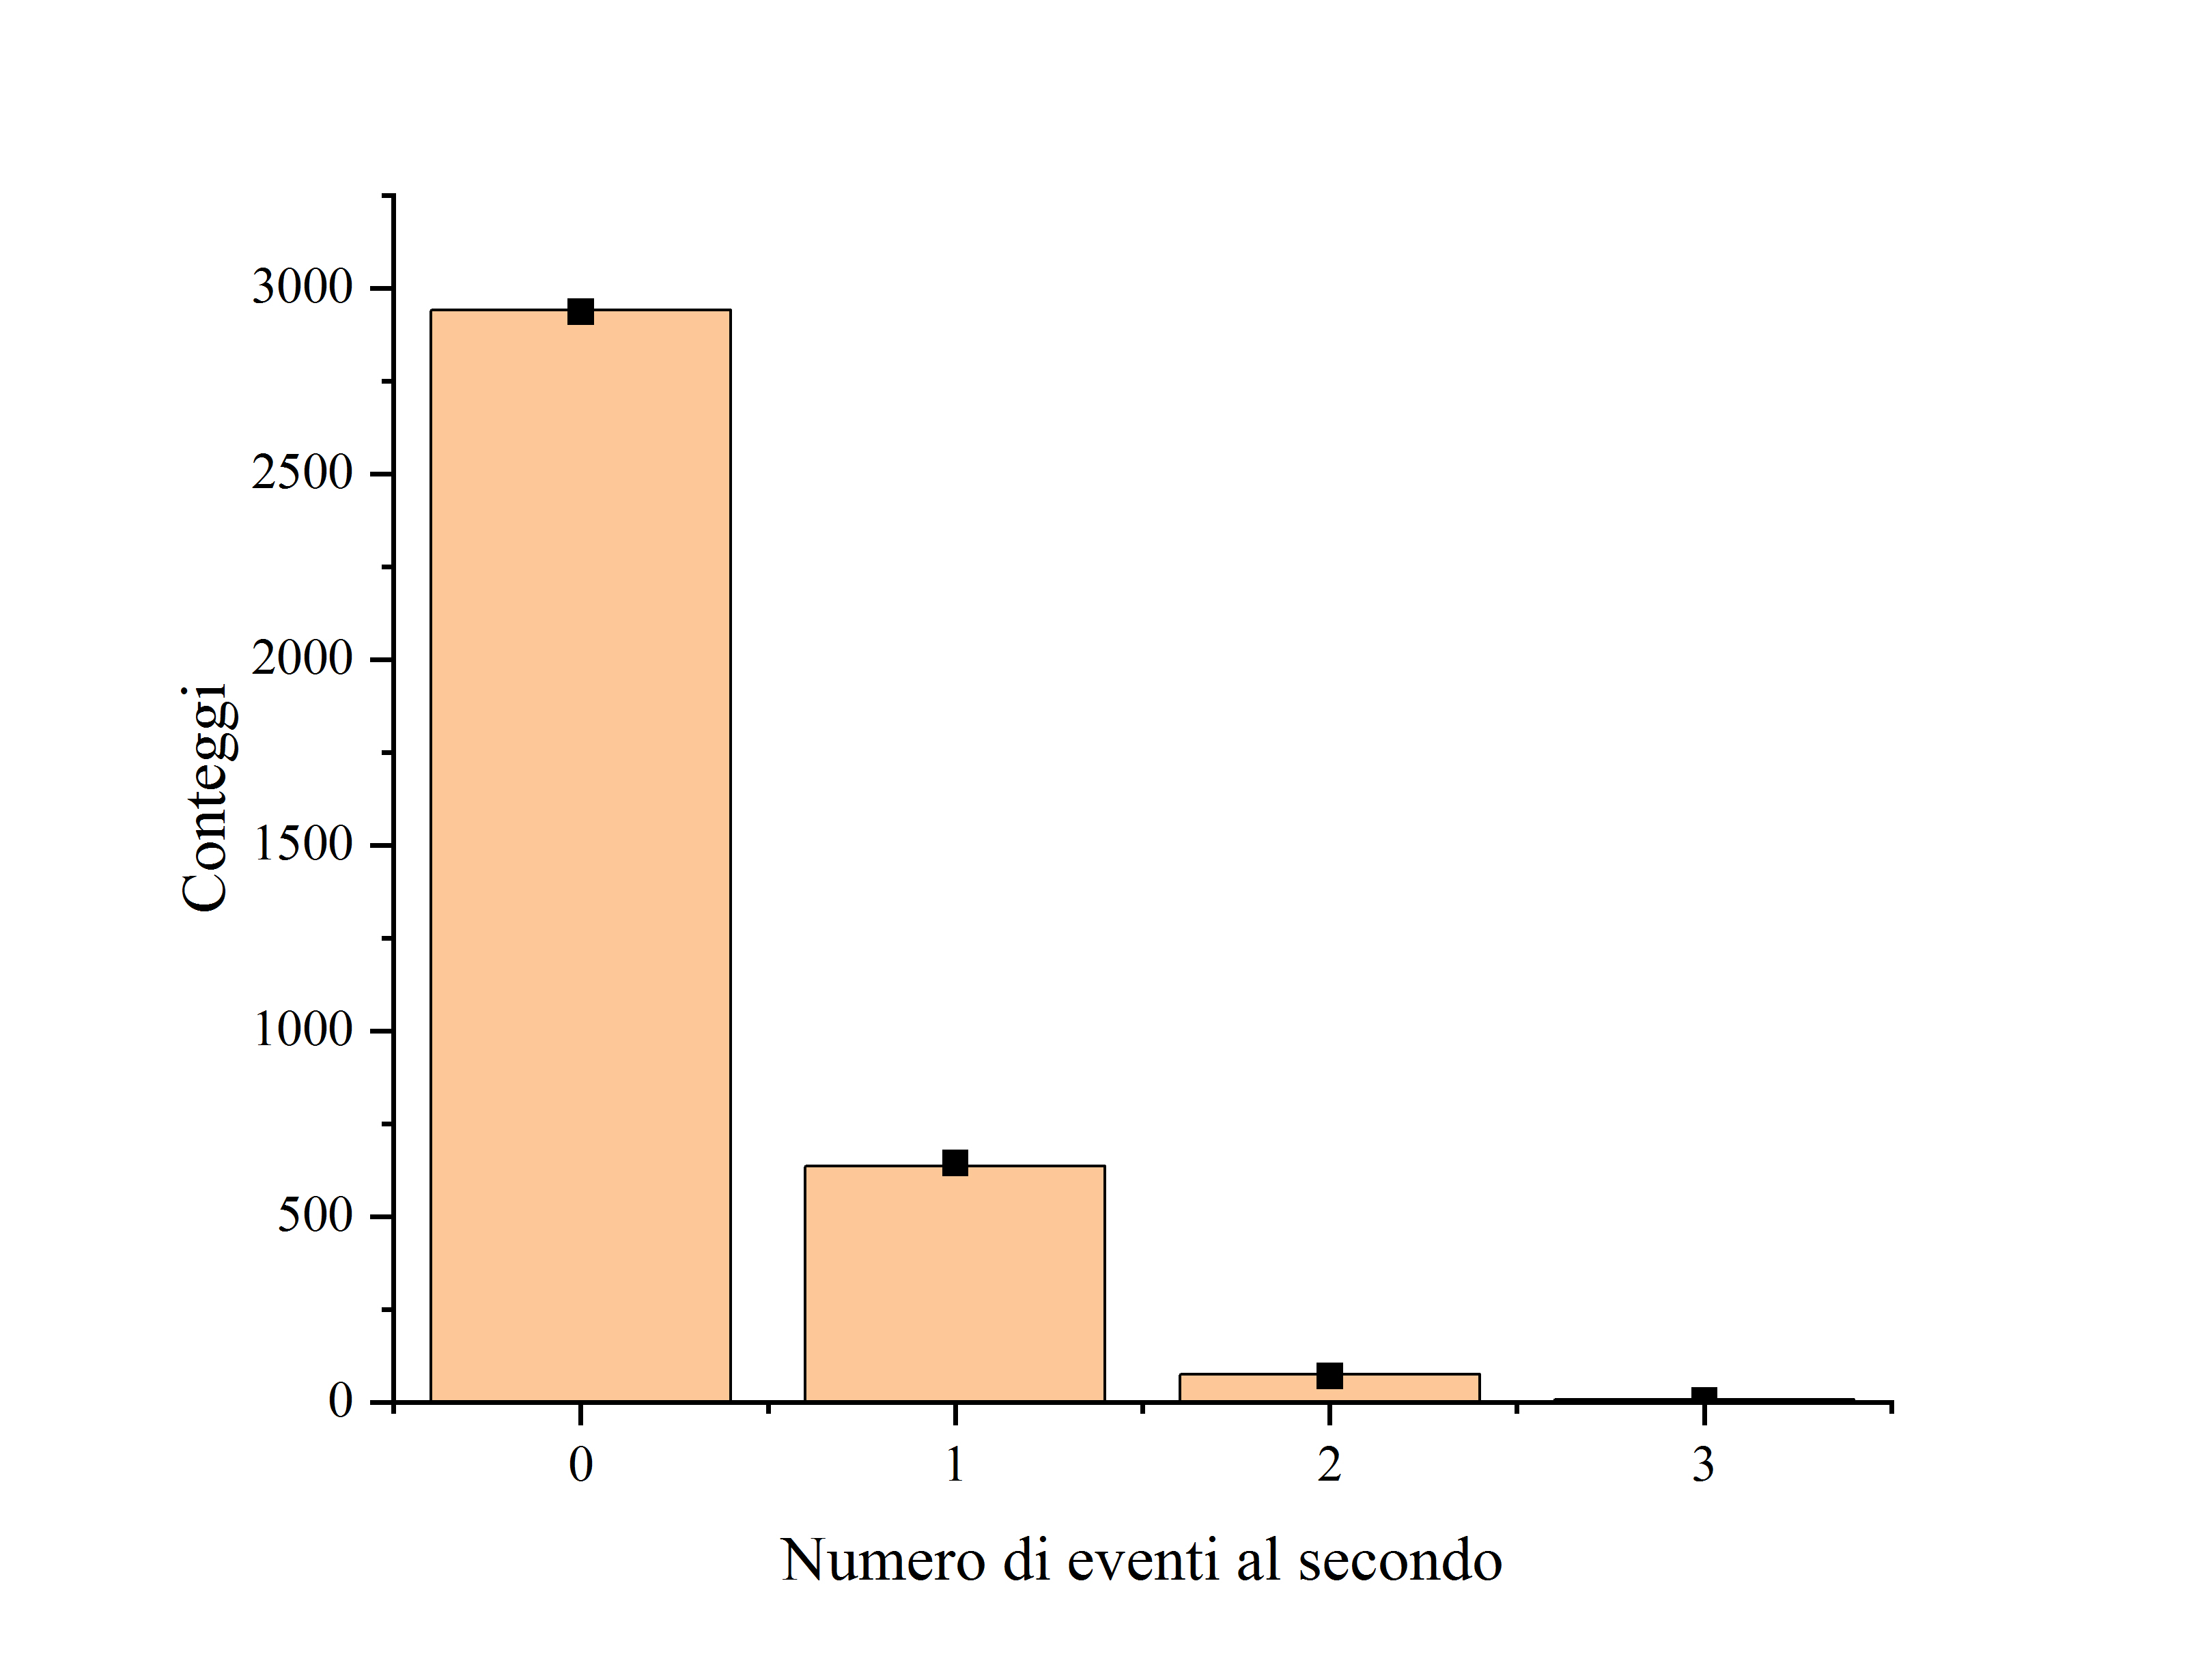
\includegraphics[trim={2cm .5cm 2.4cm 2.1cm},clip,width=.5\textwidth]{img/Geiger5.jpg}
        \caption{
            Istogrammi dei dati raccolti (nell'ordine, $\gamma_1$, $\gamma_2$, $\gamma_3$ e $\gamma_4$).\\
            I quadratini neri rappresentano i valori delle rispettive distribuzioni teoriche.
        }
    \end{figure}
    \vspace{.5cm}
    \begin{tblr}{ |Q[c,m]|Q[c,m]|Q[c,m]|Q[c,m]| }
        \hline
        $i$ & $d_i\;\;(\unit{cm})$ & $d_i^{-2}\;\;(\unit{m^{-2}})$ & $\overline{\gamma_i}$ \\
        \hline
        1 & $9.5\pm0.1$  & $111\pm2$      & $0.809\pm0.015$\\
        2 & $10.3\pm0.1$ & $94.3\pm1.8$   & $0.737\pm0.014$\\
        3 & $26.5\pm0.1$ & $14.24\pm0.11$ & $0.272\pm0.009$\\
        4 & $41.2\pm0.1$ & $5.89\pm0.03$  & $0.219\pm0.008$\\
        \hline
    \end{tblr}
    \begin{figure}[H]
        % trim={< v > ^}
        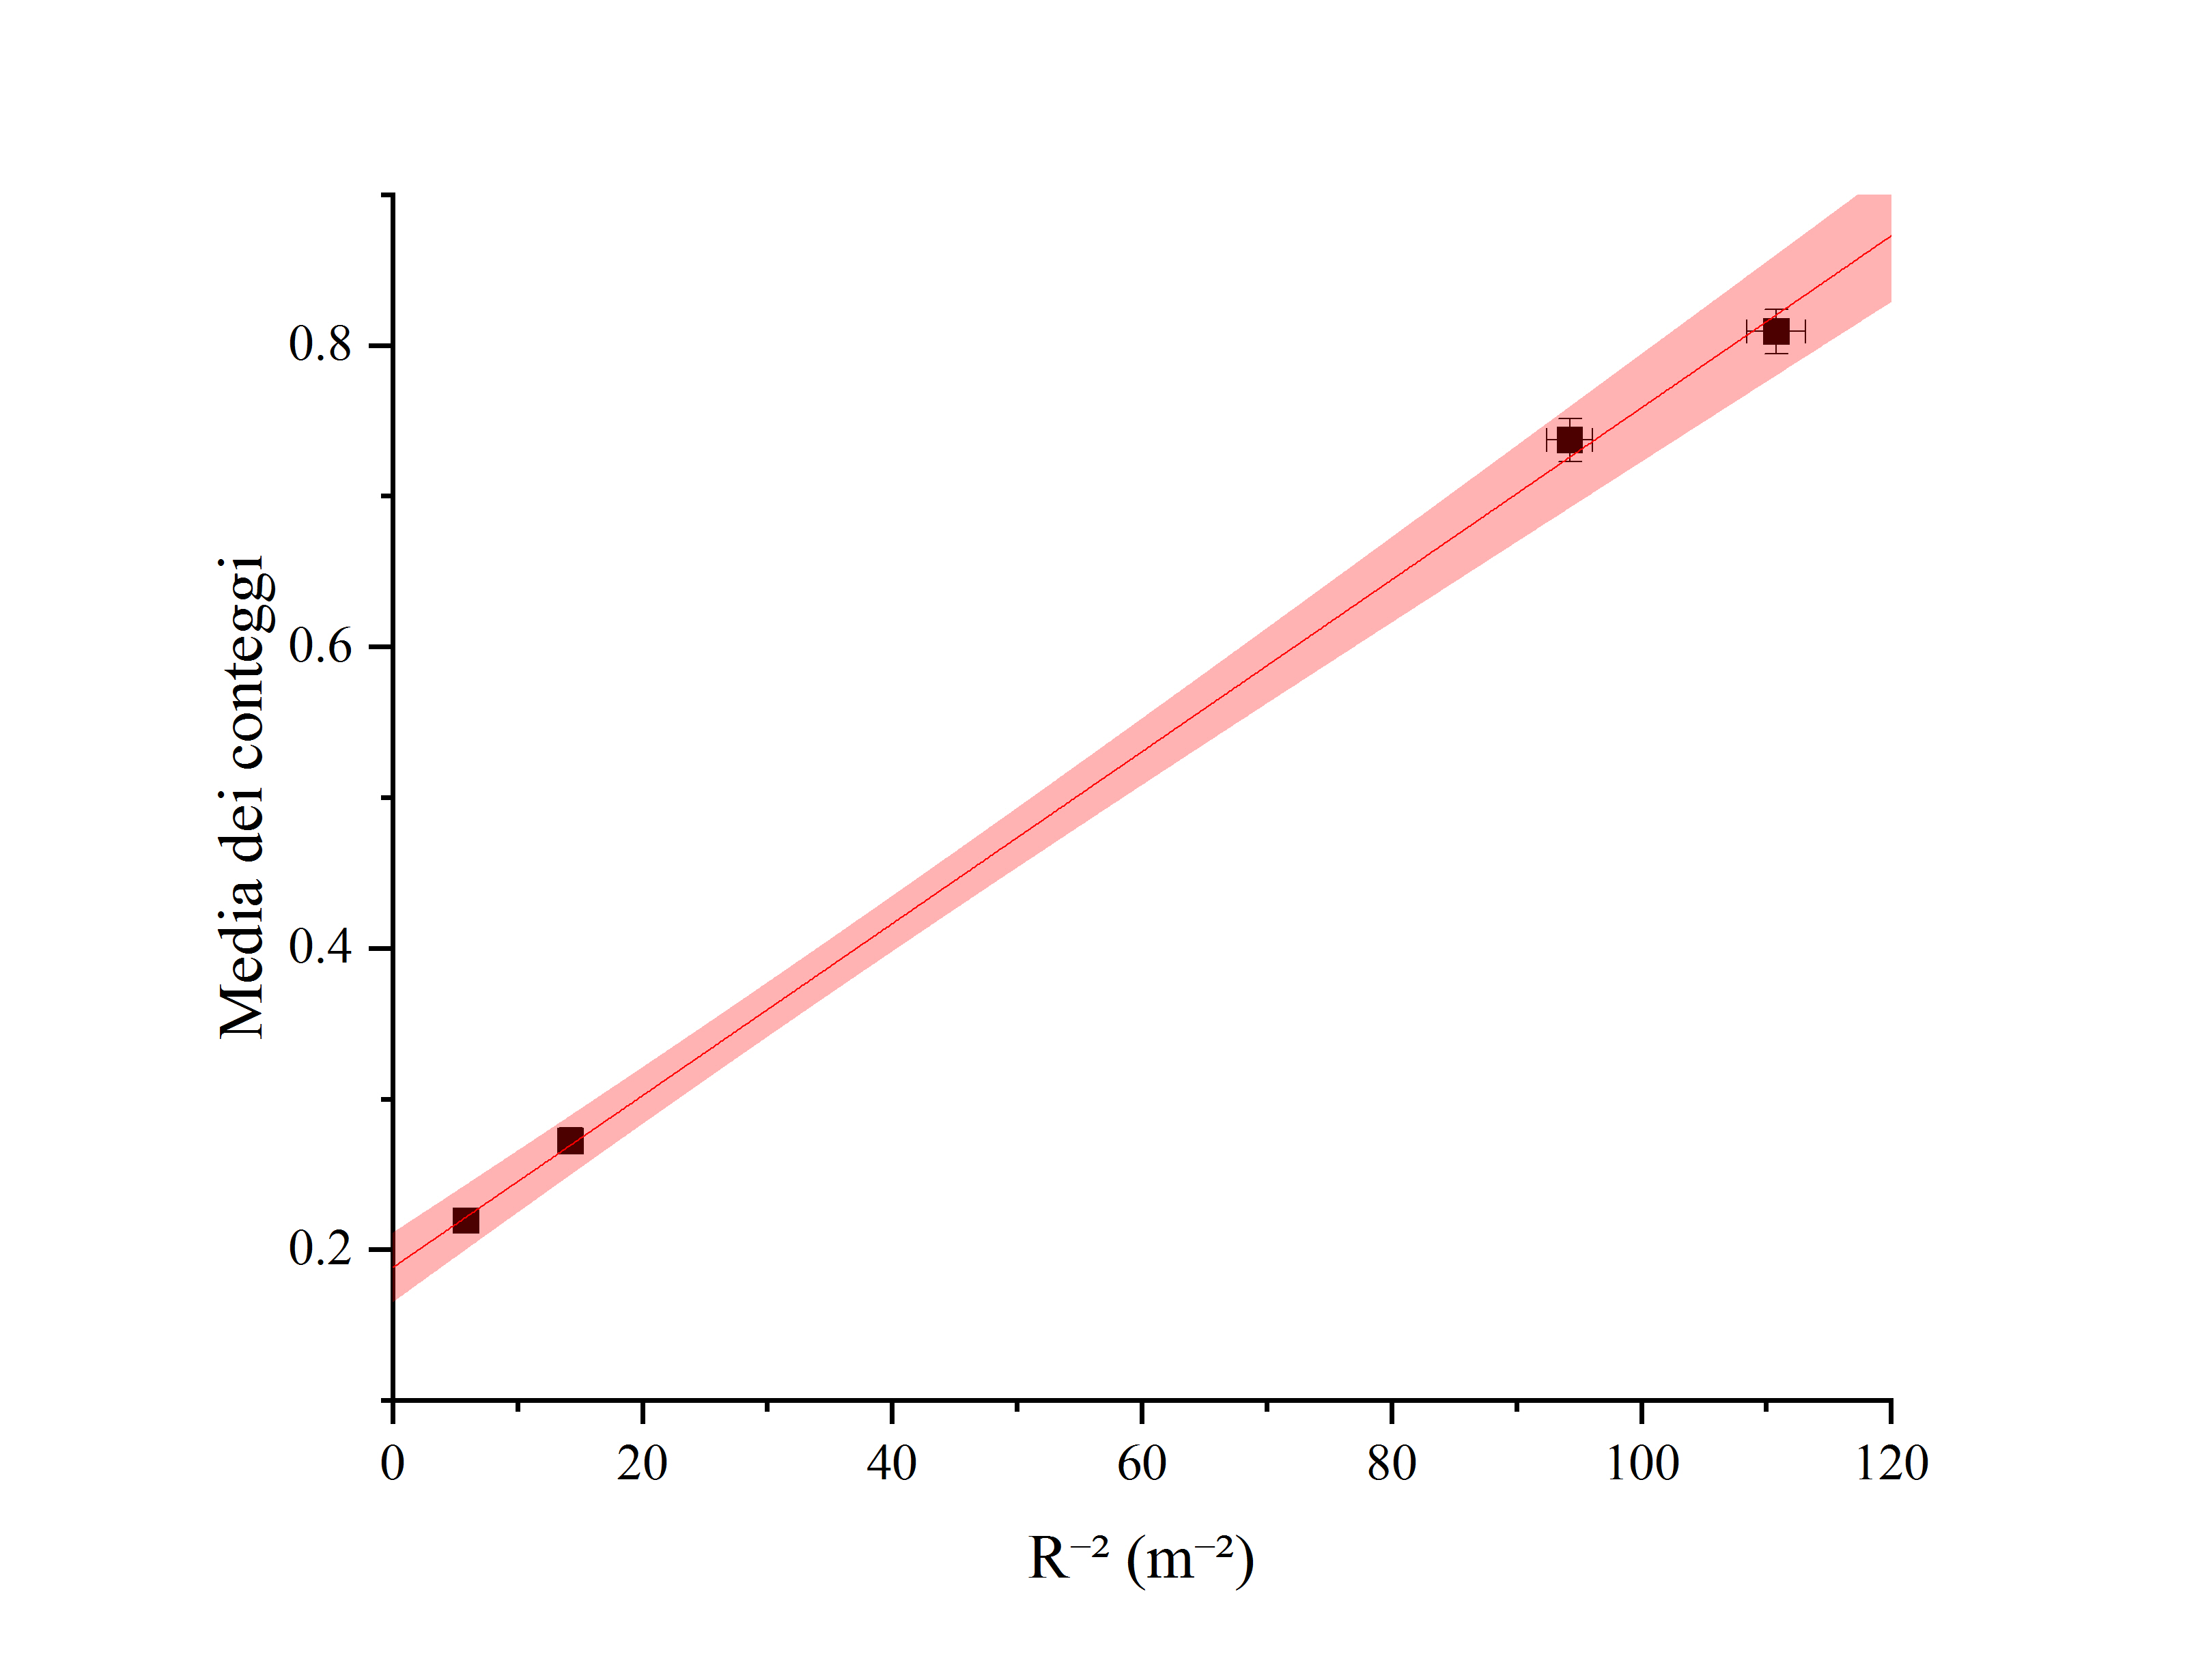
\includegraphics[trim={2cm .5cm 2cm 2.1cm},clip,width=\textwidth]{img/Regressione.jpg}
        \caption{
            La retta di regressione (in rosso) e la sua regione di incertezza (in rosa, appena visibile).
        }
    \end{figure}
\end{center}

\subsection{Conclusioni}
Per valutare numericamente la consistenza tra i due valori di $k$ ottenuti,
abbiamo calcolato il seguente valore (numero puro):
\[
    \varepsilon =
    \frac{
        \left|\left(k_\text{statica}\right)_\text{best} - \left(k_\text{dinamica}\right)_\text{best}\right|
    }{
        \delta k_\text{statica} + \delta k_\text{dinamica}
    }
\]
Allora $k_\text{statica}$ e $k_\text{dinamica}$ sono consistenti se e solo se $\varepsilon \le 1$.

Nel nostro caso, $\varepsilon = 1.33$. Il gruppo di lavoro ha ipotizzato che
questa inconsistenza (comunque contenuta, seppur non trascurabile) fra le due
misure possa essere ragionevolmente giustificata dalla difficoltà incontrata
nel ridurre al minimo le oscillazioni in direzione perpendicolare a $\vec{g}$;
considerato inoltre che la posizione dei fototraguardi non era ottimale, ciò
potrebbe avere ulteriormente influenzato la distribuzione dei tempi. È in
effetti possibile osservare che le distribuzioni da noi ottenute non sono,
il più delle volte, del tutto simmetriche: la moda sembra essersi spostata
leggermente a sinistra – un possibile sintomo dell'influenza di un
errore sistematico sulle misure.

\pagebreak
\begin{appendices}
    \section{Codice Rust per $\cdot10^{12}$ lanci di sei dadi}
    Qui riportiamo il codice Rust, da noi scritto, che ci ha permesso di
    lanciare virtualmente $6\cdot10^{12?}$ dadi in maniera estremamente
    efficiente.

    \inputminted[linenos, mathescape]{rust}{src/main.rs}
\end{appendices}

\end{document}
